\begin{figure*}[!t]
    \centering
    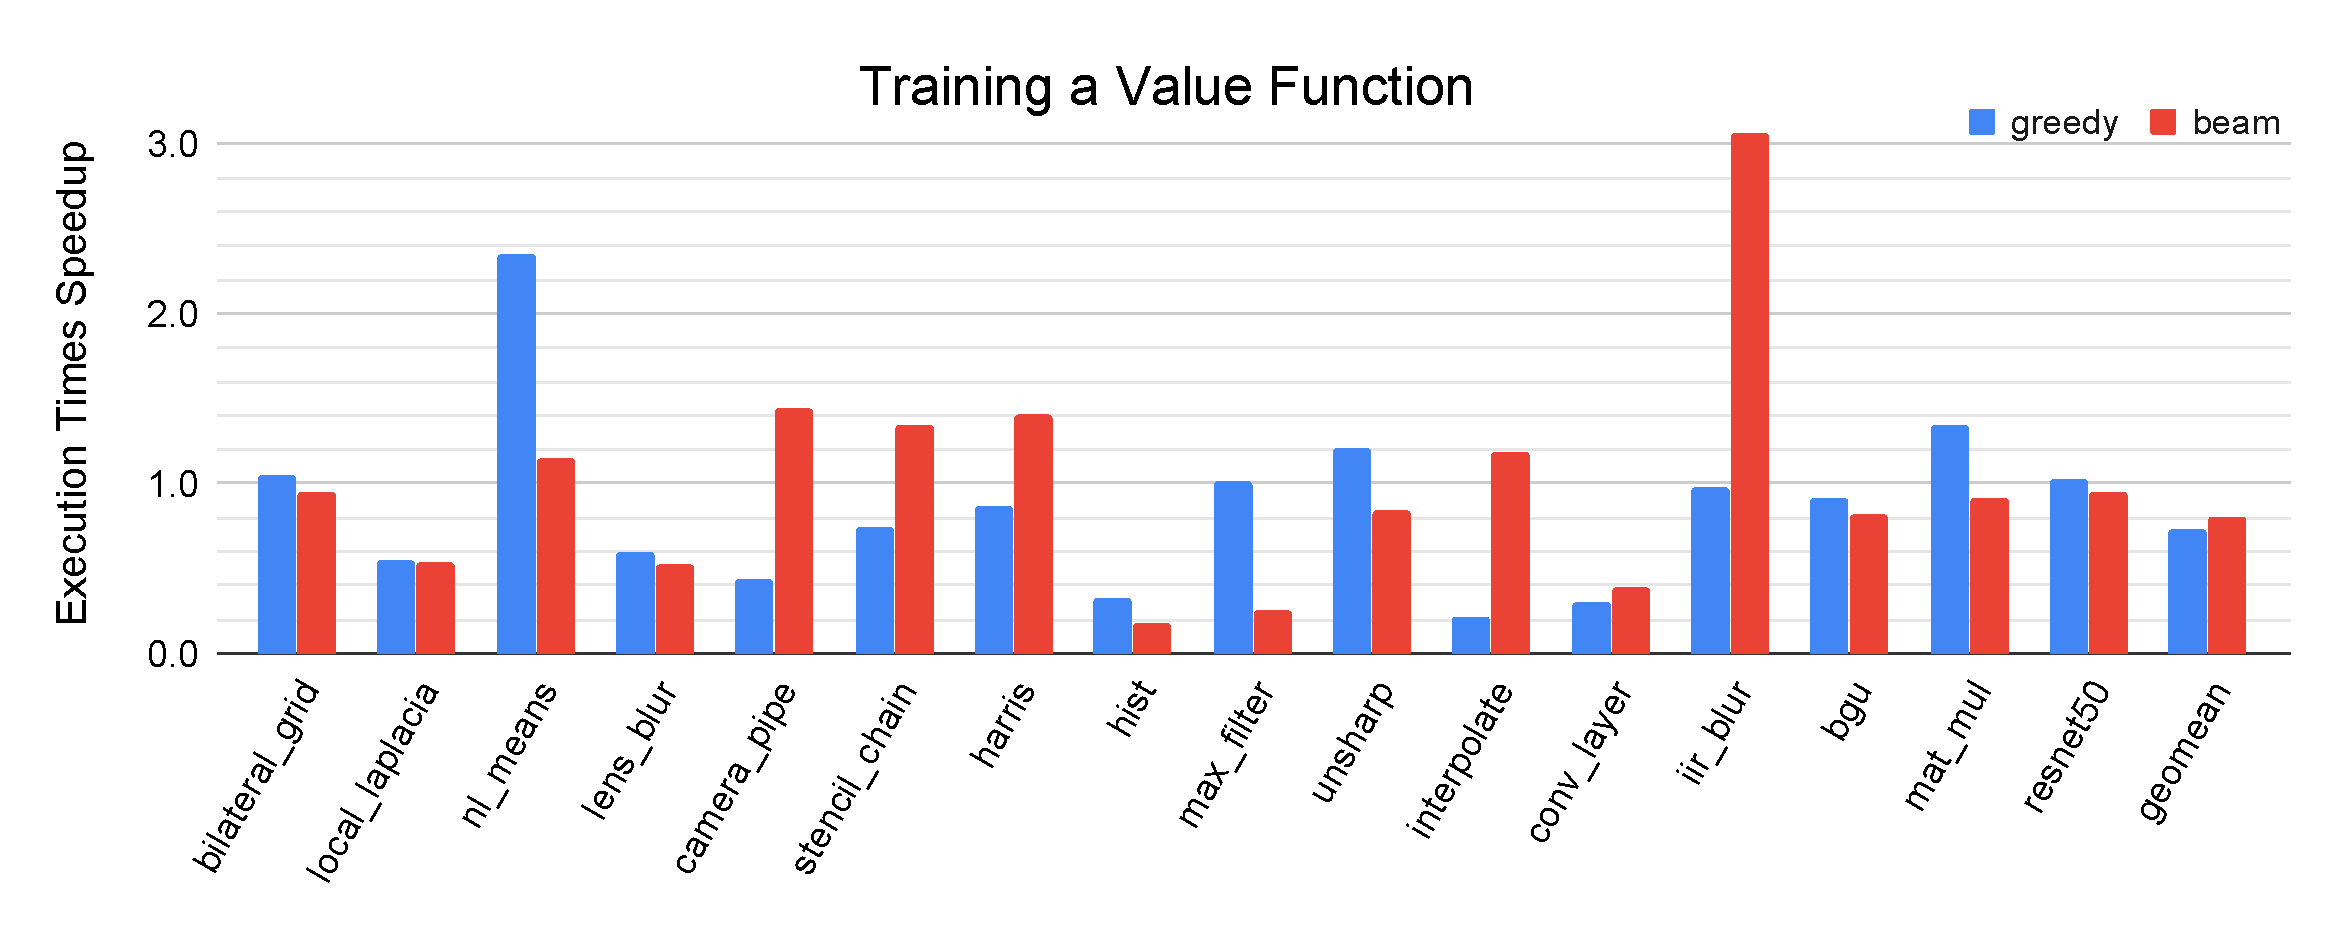
\includegraphics[trim={0cm 1cm 0cm 0cm},width=\textwidth,clip]{figures/training-value-func.pdf}
    \caption{Speedup of greedy and beam search with a cost model trained to predict the cost of the future complete schedules normalized to greedy and beam search respectively with the original cost model (trained on complete schedules only).}
    \label{fig:valuefunc}
\end{figure*}

\begin{figure*}[!t]
    \centering
    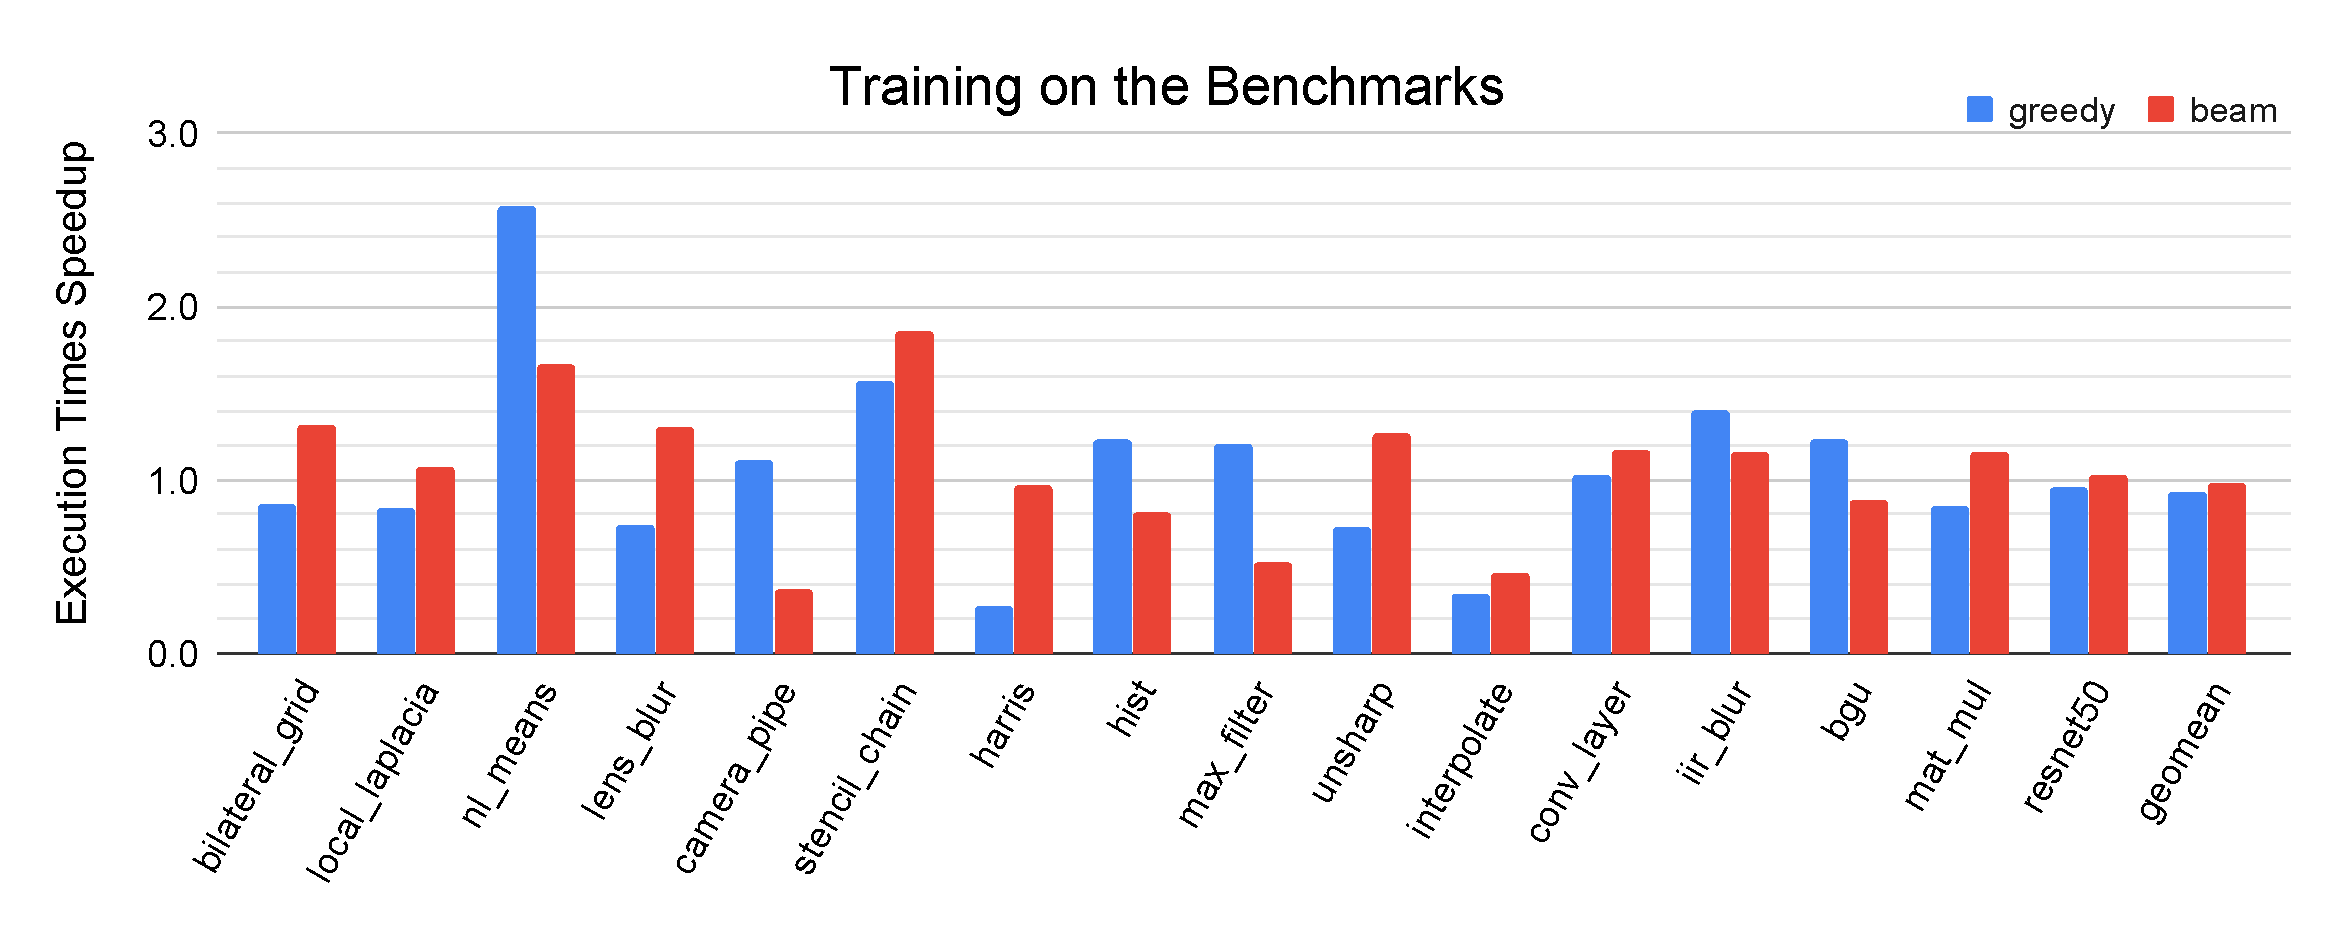
\includegraphics[trim={0cm 1cm 0cm 0cm},width=\textwidth,clip]{figures/training-on-benchmarks.pdf}
    \caption{Speedup of greedy and beam search with a cost model trained directly on random schedules of all the benchmark algorithms themselves, normalized to greedy and beam search respectively with the original cost model (trained on complete schedules only).}
    \label{fig:trainedbenchmarks}
\end{figure*}

\section{Challenges in Beam Search}

%As beam search only selects the most fit nodes to explore, beam search is an example of a greedy algorithm. It is well known that the use of greedy search algorithms fail to find the optimal solution if the state space has local maxima. Moreover, even without any local maxima, greedy algorithms will fail to find the best solution given a budget on the number of actions~\cite{shavit2019extracting}.

A beam search-based approach~\cite{adams2019learning} has been recently proposed as a scheduler in Halide, which achieves state-of-the-art results. In this approach, a cost model is trained as a proxy for predicting the true execution time of intermediate schedules used by the beam search to determine which schedules to take. Unfortunately, the cost model is trained on fully scheduled programs and cannot predict the execution time of incomplete/partially-scheduled programs. We also observed that the cost model often falls short in properly predicting execution times of fully scheduled programs and thus often minimal cost does not necessarily mean optimal execution time. This makes the beam search very sensitive to inaccuracies in the cost model. Since beam search queries the cost model at every scheduling decision, this error aggregates. 

We experimented with two techniques to overcome the challenge of predicting the execution time of incomplete programs. In the first we trained a cost model as was done in~\cite{adams2019learning}, except that we trained it on the fully scheduled benchmarks that we later run the search on. Figure~\ref{fig:trainedbenchmarks} shows the results on beam search and greedy search (beam size of one) with the new cost model. We observe that the performance improves for some benchmarks while for others it deteriorates and overall the performance is similar. This was also observed by the authors in~\cite{adams2019learning} when they retrained their cost model on the specific benchmark programs that they were also autotuning. The reason is that even if the model is trained on the benchmarks that we later run the inference on, it is hard for the cost model to accurately predict the execution time of incomplete schedules during the search. In the second experiment shown in Figure~\ref{fig:valuefunc} we trained the model to predict the future cost of the current schedule. This also did not work well because there are multiple options for scheduling the rest of the program and thus the same partial schedule of a program can lead to different costs.
%These theoretical results directly translate to the need for non-greedy algorithms in scheduling. %Consider the code snippet in Figure~\ref{fig:intermediate}. Given two possible actions -- to either split or parallelize the loop, a greedy scheduler would parallelize the loop as it would result in a likely performance gain whereas the split would leave the runtime mostly the same. However, first splitting the loop then parallelizing it would result in a better runtime as it is able to reduce the overhead from the parallel loop.

% \begin{figure}
%     \centering
%     \begin{minted}{c}
% for(int i=0; i<n; i++) {
%     out[i] = in[i];
% }
%     \end{minted}
%     \caption{Original code to schedule.}
%     \label{fig:intermediate}
% \end{figure}

% \begin{figure}
%     \centering
%     \begin{minted}{c}
% parallel_for(int i=0; i<n; i++) {
%     out[i] = in[i];
% }
% \end{minted}
%     \caption{Applying a parallel for.}
%     \label{fig:par}
% \end{figure}


% \begin{figure}[!t]
%     \centering
%     \begin{minted}{c}
% for(int i=0; i<n; i+=10) {
%     for(int j=i; j<i+10; j++)
%         out[j] = in[j];
% }
% \end{minted}
%     \caption{Splitting the loop.}
%     \label{fig:split}
% \end{figure}


% \begin{figure}
%     \centering
%     \begin{minted}{c}
% parallel_for(int i=0; i<n; i+=10) {
%     for(int j=i; j<i+10; j++)
%         out[j] = in[j];
% }
% \end{minted}
%     \caption{Parallelizing the outer loop.}
%     \label{fig:split}
% \end{figure}



To overcome these challenges we formulate the scheduling problem as an MDP. In such a framework, a graph node represents an intermediate schedule/program, with edges between nodes representing potential scheduling actions. Thus, applying a particular schedule to a program could be seen as a simple graph traversal. Algorithms that solve such MDP's seek to find a node/set of actions that maximize the reward of the end state. In our use case, the reward would be the inverse of the execution time (thereby ensuring that maximizing the reward gives the fastest program).

MCTS is a promising algorithm for solving MDPs. We chose to use MCTS for four reasons: it is theoretically guaranteed to find the best node with sufficient time; its UCB formula balances the exploration of new states and exploitation of existing good states combined with using the expectation of future rewards which makes it more resilient to noise; its ability to look ahead before making a decision avoiding greediness; and the ability to make decisions based on costs of fully scheduled programs, which means the cost model can predict their execution time more accurately. Furthermore, MCTS allows us to combine real execution time measurements and the cost model's predictions to further improve performance.
%This is vital as evaluating the cost is quite expensive, and as shown in Table \ref{tab:Beambreakdown} evaluating the cost represents 92.3\% of their runtime. However, as we found in Section~\ref{}, ther

%We have chosen the use of a Monte Carlo Tree Search (MCTS) for three reasons: it has a theoretical guarantee to find the best node with sufficient time; its upper confidence bound (UCB) formula that balances exploration of new states and exploitation of existing good states is rather resiliant to noise\wmnote{cite};  and in practice MCTS only spends only 22.1\% of its runtime evaluating the cost model, compared to 92.3\% in beam search, allowing us to use more expensive cost models without as dramatic of a performance penalty.

% \wmnote{We want to also probably see how many of our choices made in practice are greedy vs not greedy choices.}

% \wmnote{The perf analysis really doesn't seem like it should go here, also should be formatted nicer}

% \begin{table}[!t]
% \centering
% \begin{tabular}{|l|l|l|l|}
% \hline
% \textbf{Algorithm} & & & \\ \hline
% MCTS & 100\% & &\\ \hline
% & generate\_actions & 81.4\% &\\ \hline
% &  & compute\_features & 68.9\%\\ \hline
% &  & calculate\_cost & 9.7\%\\ \hline
% &  & other (memory/etc) & 2.8\%\\ \hline
% & evaluate\_cost & 11.6\% &\\ \hline
% & other & 7.0\% &\\ \hline
% \end{tabular}
% \caption{Performance breakdown of MCTS on Local Laplacian test.}
% \label{tab:MCTSbreakdown}
% \end{table}


% \begin{table}[!t]
% \centering
% \begin{tabular}{|l|l|l|l|}
% \hline
% \textbf{Algorithm} & & & \\ \hline
% Beam & 100\% & &\\ \hline
% & generate\_actions & 91.9\% &\\ \hline
% &  & compute\_features & 2.6\%\\ \hline
% &  & calculate\_cost & 88.3\%\\ \hline
% &  & other (memory/etc) & 1.0\%\\ \hline
% & evaluate\_cost & 4.6\% &\\ \hline
% & other & 3.5\% &\\ \hline
% \end{tabular}
% \caption{Performance breakdown of Beam on Local Laplacian test.}
% \label{tab:Beambreakdown}
% \end{table}
